\documentclass[a4paper,11pt,twoside,openright]{book}


\usepackage[utf8]{inputenc}
%\usepackage[vietnam.english]{babel}

\usepackage[T1]{fontenc}




%\usepackage[Latin1]{inputenc}       %caractËres accentuÈs et autres
%\usepackage[T1]{fontenc}            %cÈsure des mots accentuÈs
%\usepackage[frenchb]{babel}         %francisation (chapitre,annexe,rÈfÈrences...)
\usepackage{graphicx}               %insertion graphiques
\graphicspath{{images/}}
\usepackage{float}
\usepackage{a4wide}
\usepackage[super]{nth}
\usepackage{mathtools}
\usepackage{hyperref}
%\usepackage{psfig}


%\psfigurepath{}




%\usepackage{times}


%\input{transfig}



\renewcommand{\thefootnote}{}

%% Necessaire pour creer les index
\usepackage{makeidx}
\makeindex





%%%%%%%%%%%%%%%%%%%%%%%%%%%%%%
%%%% MODIFY THIS PART FOR THE FIRST PAGE

% change the master level 
\def\MasterLevel{Master Thesis }
%\def\MasterLevel{Master 1}

\def\InternshipTitle{[Title of internship]}
\def\FirstName{Khoa}
\def\LastName{Nguyen Nhu}
\def\HostOrganization{ICTLab-USTH}
\def\CityName{Hanoi}
\def\CountryName{Vietnam}
\def\UniversityName{[University name]}
\def\Supervisor{Dr. Tran Giang Son}



\setlength{\textwidth}{175mm}
%
\setlength{\textheight}{245mm}

\setlength{\topmargin}{-10mm}

\setlength{\evensidemargin}{-8mm}

\setlength{\oddsidemargin}{-8mm}

% ----------------------- DEBUT DOCUMENT ---------------------------

\begin{document}



\pagestyle{plain}



\pagenumbering{Roman}


% ----------------- DEFINITION DU TITRE ET DES AUTEURS ---------------------------

\newpage
\empty
\thispagestyle{empty}

\begin{center}




%\includegraphics[angle=0,width=5cm]{images/usth-logo-final-transparent.png}



\includegraphics[angle=0,width=5cm]{logo-1_39.png}


\vspace*{1cm} 



{\huge University of Science and Technology of Hanoi }\\


\vspace*{1cm} 


{\large Information and Communication Technology Department}\\


\vspace*{1cm} 



{\huge \MasterLevel }\\


\vspace*{1cm} 

{\large Academic year 2016 -  2017}


\vfill


\noindent\hrulefill

\vspace*{2mm} 

{\Large \InternshipTitle }


\noindent\hrulefill





\vfill 



{\large presented by } \\

\vspace*{5mm} 


{\large \bf \FirstName~  \LastName} \\


\vspace*{5mm} 


%{\large registered at \UniversityName } \\



%\vspace*{5mm} 



{\large supervised by  \Supervisor } \\


\vspace*{20mm} 




{\large Host organization :   \HostOrganization }


\vspace*{5mm} 


{\large  \CityName~- \CountryName} \\

\vspace*{5mm} 





%\noindent\hrulefill


\end{center}


% ----------------------- PAGE VIDE ---------------------------




\chapter*{ATTESTATION}



\vfill


\noindent\hrulefill

~\\


I hereby,  \FirstName~  \LastName, certify that my report doesn't contain plagiarism (copy/paste) from other sources.

~\\

In case of plagiarism in my report, I know the consequences and I understand that my report won't be evaluated. In this case, my M1 internship will be noted as "fail".


~\\

 Date 

~\\
 
 Signature 
 ~\\

 \FirstName~  \LastName
 

~\\
~\\
~\\
~\\
~\\

\noindent\hrulefill


\vfill


\vfill



%\selectlanguage{vietnam}
%
%
%Tôi ký tên dưới đây, <họ> <tên>, xác nhận rằng bài báo cáo của tôi không có đạo văn (lỗi sao chép) từ các nguồn khác.
%
%
%~\\
%
%
%Nếu bị phát hiện ra trong bài báo cáo, tôi biết hậu quả và tôi hiểu rằng bài báo cáo của tôi sẽ không được chấp nhận. 
%Trong trường hợp đó, học phần (thực tập năm thứ nhất, thực tập năm thứ hai, hay học phần đánh giá) sẽ bị ghi là “không đạt”.
%
%
%
%~\\
% 
%Ngày … tháng … năm …
% 
%
%~\\
% 
%Chữ ký
%
%
%~\\
%~\\
%~\\
%
%
%\selectlanguage{english}
%
%\noindent\hrulefill




\setcounter{page}{1}



% ----------------------- ACKNOWLEDGEMENTS ---------------------------

\chapter*{Acknowledgements}

First and foremost, I would like to express my deepest gratitude to Dr. Tran Giang Son, my research supervisor for his patience, helpful theoretical and practical advice and enthusiastic encouragement during the period of my internship. \\
Second, I am grateful for all the support along the internship period of Assoc. Prof. Ngo Duc Thanh and Assoc. Prof. Damien Gratadour\\
Also, I want to thank the University of Science and Technology of Hanoi (USTH) in general and specifically, the USTH ICTLab for granting me this opportunity to work as one of the temporary member of the lab. \\
Last but not least, I would like to appreciate the support from my family and friends during my internship. \\





% ----------------------- RESUME ---------------------------


\chapter*{Asbtract}

In recent years, parallel computing has become more popular, with the advancement of hardware, such as multicore processor, and the development of parallel architecture. Nowadays, parallization exists in many places, such as modern day PC/Workstation, Cluster, Grid Computing system or High Performance Computing system in general. This is due the demand for enhancement in computing performance to solve enormous, complex problem. \\
The main focus of the intership is to investigate potential improvement for the Regional Climate Model with GPU and parallelization, and provide some proofs of concept for this matter. Testing will be conducted using OpenMP Parallel API.\\
~\\
Keyword: Parallel Computing, OpenMP, Regional Climate Model, High Perfomance Computing

% ----------------------- PAGE VIDE ---------------------------


% ----------------------- REMERCIEMENTS ---------------------------

%\include{Thanks}

% ----------------------- TABLE DES MATIERES ---------------------------



\tableofcontents{}


\newpage


\listoffigures{}

\newpage

\listoftables


\newpage



\chapter*{List of Abreviations}


\newpage




% ----------------------- TABLE DES FIGURES ---------------------------
%\listoffigures{}

% ----------------------- TABLE DES TABLES ---------------------------
%\listoftables{}

% ----------------------- TABLE DES TABLES ---------------------------
%\listoflistings{}

% ----------------------- CHAPITRE ---------------------------
\pagenumbering{arabic}

\chapter{Introduction}

\section{Context and Motivation}

Climate models are representations of factors that have impacts on climate, described by mathematical equations based on the law of physics. Main factors that can affect the climate are the atmosphere, oceans, living creatures, land exterior, ice, and energy produced by the Sun. Together with other sophisticated elements such as cloud, rainfall, water evaporation, etc., these climate models are put into use in order to achieve various objectives such as studying the tendencies of climate systems or estimating future climate ~\cite{climate_modeling}. Not only incoming energy emitted from the sun, as mentioned above, is taken into consideration in the form of short-wave electromagnetic radiation, but also outgoing long-wave infrared electromagnetic one. With both of these radations are taken into account, any changes that cause imbalance between the two will result in a change in temperature, thus changing the climate. ~\cite{jana_majumder_2011}. \\
~\\
Climate models, with the way their data and computations are processed, have benefited greatly from exploiting parallelism, especially with vector processors and the recently extended Single Instruction Multiple Data parallel paradigm. However, most of the climate models today are computed in cluster-based computer with large, powerful microprocessors, which are unable to fully utilize parallelism to a greater extent. This is due to the fact that CPUs lack the necessary memory bandwidth to obtain such level of parallelism, no matter how powerful the CPU can be.\\
~\\
University of Science and Technology of Hanoi (USTH) research lab REMOSAT, led by Assoc. Prof Ngo Duc Thanh, has been in urgent need for perfomance boost and computation time acceleration of the climate models running in the lab, specifically, the Regional Climate Model system, or RegCM for short. In this context, the goal of the internship is to investigate possible usage of GPU in climate models simulation performed by the REMOSAT research lab to speed up its processing time.\\

\section{Regional Climate Model system (RegCM)}

The Regional Climate Model system, also known as RegCM, unlike other global climate models, was developed using Fortran as a limited area model for the purpose of long term simulation in specific regions. RegCM is meant to be used as a public, open source software that is user-friendly and portable enough to be apply in any domains in the world. Being a community model, and is designed to be applied in a vast number of communities, RegCM has partaken in a large number of regional climate projects, and has been aiding various climate studies and future climate predictions ~\cite{regcm_man}. \\
~\\
Originally created by the National Center of Atmospheric Research (NCAR) back in 1989, it has now evolved over time after numerous of patches and a few major updates. As of the most recent release, RegCM4, the program contains many upgrades and new features compare to previous versions. Most noticably, RegCM has now improved on flexibility, portablity and user friendliness, and is now fully supported by the Earth Physics System, as the developers commented in the Documentation ~\cite{regcm_ictp}. \\
~\\
A typical run of Regional Climate Model system consists of two main parts. First, based on the global dataset, the system will generate input data for the simulation, including the domain of simulation, sea surface temparature, initial condition, boundary condition, and other optional dataset ~\cite{regcm_man}. After being successfully produced, these input data are put in the RegCM program to run the simulation. It is worth mentioning that RegCM supports Open Message Passing Interface(OpenMPI), which is a standard API for parallel/distributed computing built on the Message Passing parallel model. Upon completing, the program will generate output models of the simulation, containing information on atmosphere status, surface diagnostic variables, radiation fluxes, and a save point that holds the model's status at the end of the run, which enables the simulation to restart at that point, thus allowing the user to split a long simulation into much many shorter ones. \\

\section{Limitation of RegCM}

While having full OpenMPI support, meaning that it can run simulation in parallel using the Message Passing parallel paradigm, RegCM still has some limitations in its parallelism. First and foremost, since the method of implementing parallelization is OpenMPI, CPU-based parallelism is utilize while running simulations, which imply the above mention restriction about lack of memory bandwidth, especially when parallel processes need to exchange data with each other. Moreover, CPU parallelization limits the number of processes can run simutaneously to no more than the number of logical cores the CPU has, which can hurt the performance on lower core count CPUs. Another drawback that the developers have pointed out regarding RegCM's parallel implementation is that it current has no form of parallel I/O, indicate that not all processes can have access to the data at the same time ~\cite{regcm_man}. \\

\section{Host Institution}

ICTLab of University of Science and Technology of Hanoi (USTH) is a joint international research laboratory in the field of Information and Communication Technology (ICT) between USTH and other French partners. The lab has researchers from USTH, Institute of Information Technology (IOIT) of Vietnam Academy of Science and Technology (VAST), Institut de Recherche pour le Dévelopment (IRD) and the University of La Rochelle, France ~\cite{ictlab}. \\
~\\
\begin{figure}[h]
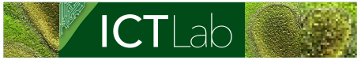
\includegraphics[angle=0,width=10cm]{ictlab_logo.png}
\centering
\caption{ICTLab Official Logo}
\end{figure}
~\\
The ICTLab was created on December 1st, 2014, supported by USTH, French Embassy in Vietnam, 13 French high education institutes and universities (namely, USTH Consortium), and the Asian Development Bank (ADB) ~\cite{ictlab}. \\
~\\
The researches of ICTLab focus on two main applicative axes: Cultural heritage preservation and promotion, and Environmental protection and Environmental risk management. Fundamental research programs target common scientific activities, such as Modeling, Image Processing and Analysis, Machine Learning, Expert User Interaction, Geographical Information Systems, Information Retrieval, and Sensor ~\cite{ictlab}. \\
~\\
Regarding to these research activities, ICTLab is currently working on two main projects. The first project, SWARMS (Say and Watch: Automated image/sound Recognition for Mobile monitoring Systems), aims to achieve a flexible and real-time monitoring network, where device can used as both passive sensors and active transmitter that can send visual, voice, textual pieces of information to a monitoring system, so that stakeholder can analyze and forecast information. The other project, ARCHIVES (Analysis and Reconstruction of Catastrophes in History within Interactive Virtual Environments and Simulations), focuses on supporting historical research on past disasters with assistance of advance document image processing and analysis, information retrieval, machine learning, Geographical Information System (GIS) representation and agent-based computer modeling ~\cite{ictlab}. \\

\section{Thesis organization}

The thesis is organized as follow. Excluding the first chapter, which is Introduction, there are 4 chapters. The \nth{2} chapter discusses about background knowledge related to general paralellization, local parallelism and high performance computing. Chapter 3 explains the methodology carried out during the internship period. Testing and result are shown in the \nth{4} chapter, and the last chapter will conclude the thesis with remarks, limitation and possible future works. 


% ----------------------- CHAPITRE ---------------------------

\chapter{Background}

\section{Parallel Computing}

\subsection{Definition}

\begin{figure}[H]
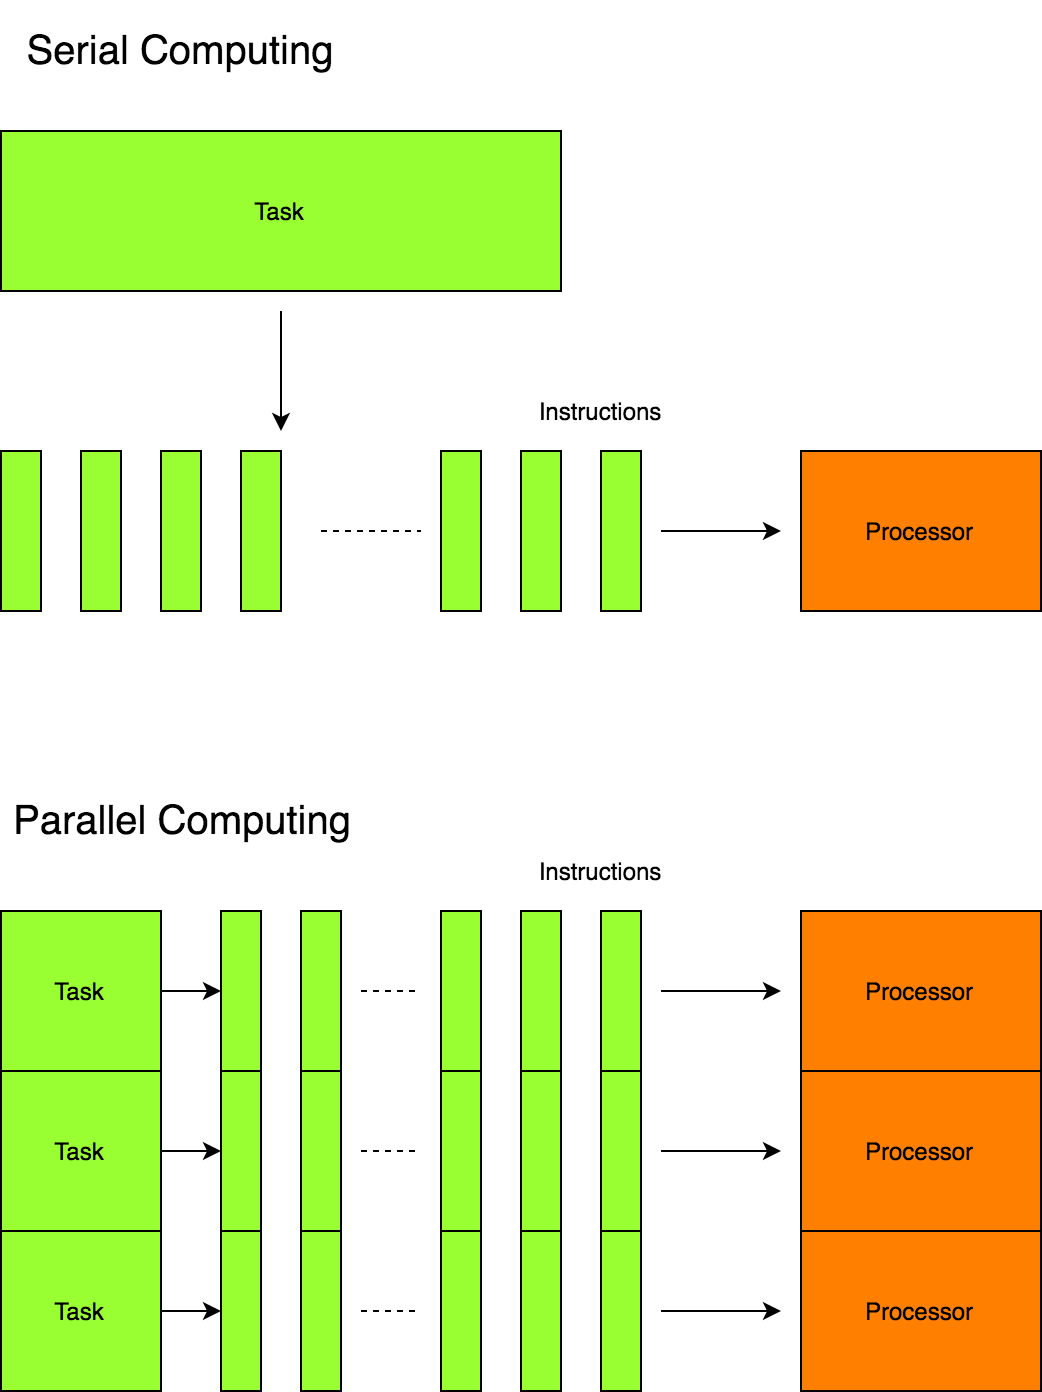
\includegraphics[width=7cm]{Parallel.png}
\centering
\caption{Comparison between Serial and Parallel Computing}
\end{figure}
~\\
~\\
Parallel computing is about executing task simultaneously based on the given computer resource to find a solution to a complex computational problem, such as modeling and simulation. Unlike the traditional serial computation, where instructions are executed in succession one at a time, in parallelization, a problem are divided into many different, disctint segments, each can be further decomposed into set of instructions. The distintion between these segments allows them to be performed on different processors in a parallel fashion. The computation resource required for parallel computing, as stated previously, can be either a powerful computer with a multiple cores/threads CPU or a network of serveral computers, with or without dedicated GPUs~\cite{intro_parallel}. \\


\subsection{Motivation}

The drive to utilize parallel computing is strongly related to real world problems, where many events, complementing each other, happen more or less simultaneously, however inside a chronological sequence~\cite{intro_parallel}. Because of how natural phenomena work and how complex they are, serial computing is not suited for heavy workload of modeling and simulating such events. Serialize computation is too time-consuming for this kind of tasks, as being only able to do one job at a time. \\
~\\
Parallel computing, on the other hand, is clearly much more fitted for this line of work. By taking advantage of computers network, whether it is a local or remote one, tapping into parallel potential within modern computer hardwares(multi-core CPU, CUDA GPU) or even both of the above at the same time, parallelization provides the power needed to not only solving mathematical problems with high level of complexity that can be impossible to run on serial computing model, but also gaining better performance time, resulted in more computation tasks can be done, hence more efficient and profitable~\cite{intro_parallel}. \\


\subsection{Flynn's taxonomy on parallel architecture}

Introduced in 1966, Michael J. Flynn, the author, suggested that high-speed computer can be divided into 4 main categories, based on Instruction Stream and Data Stream. Stream, as Flynn explained (1966), "refers to sequence of data or instructions as seen by the machine during the execution of the program". Flynn clarified further that Instruction Stream and Data Stream serve as a convenient baseline to classify computer organization while preventing any confusion driven by the term "parallelism"~\cite{flynn}. \\
\begin{figure}[H]
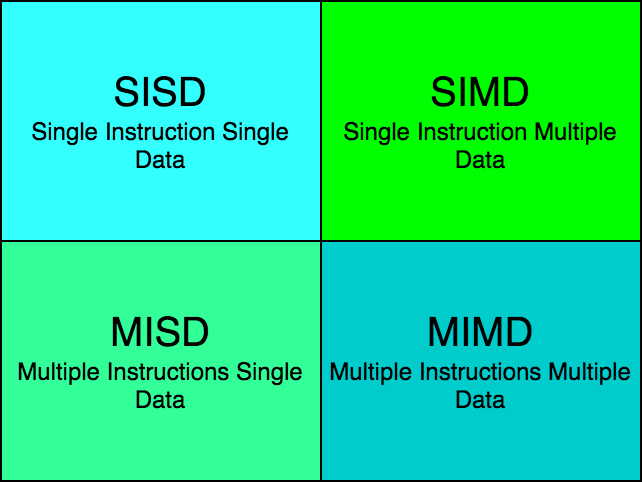
\includegraphics[width=7cm]{Flynn.png}
\centering
\caption{Flynn's taxonomy}
\end{figure}
~\\
%Some images to illustrate this
The computer organization are classified as below:
\begin{itemize}
	\item Single Instruction Stream, Single Data Stream (SISD): Also known as serial (non-parallel) computation, this is the oldest type of computer, in which the processing unit can only take one instruction stream and use one data stream as input at a time during a clock cycle~\cite{intro_parallel}.
	%Image for each kind of architectures
	\begin{figure}[H]
	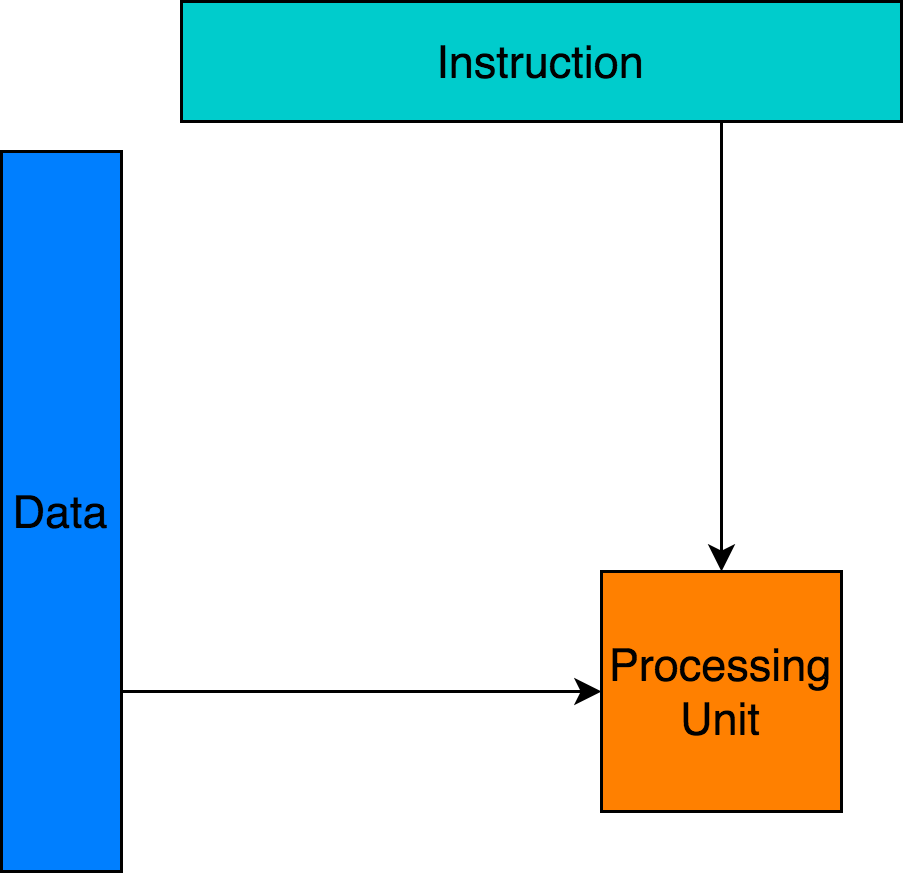
\includegraphics[width=5cm]{SISD.png}
	\centering
	\caption{Single Instruction Single Data architecture}
	\end{figure}
	\item Single Instruction Stream, Multiple Data Stream (SIMD): A popular parallel architecture (appears the most in GPU) that processing units take the same instruction stream during a clock cycle, but the data stream given to them are different from one another. An example of SIMD is image processing, where the processing unit was given one instruction stream to some(or even all) of their core/thread, handling many pixels (multiple data stream) at the same time.
	\begin{figure}[H]
	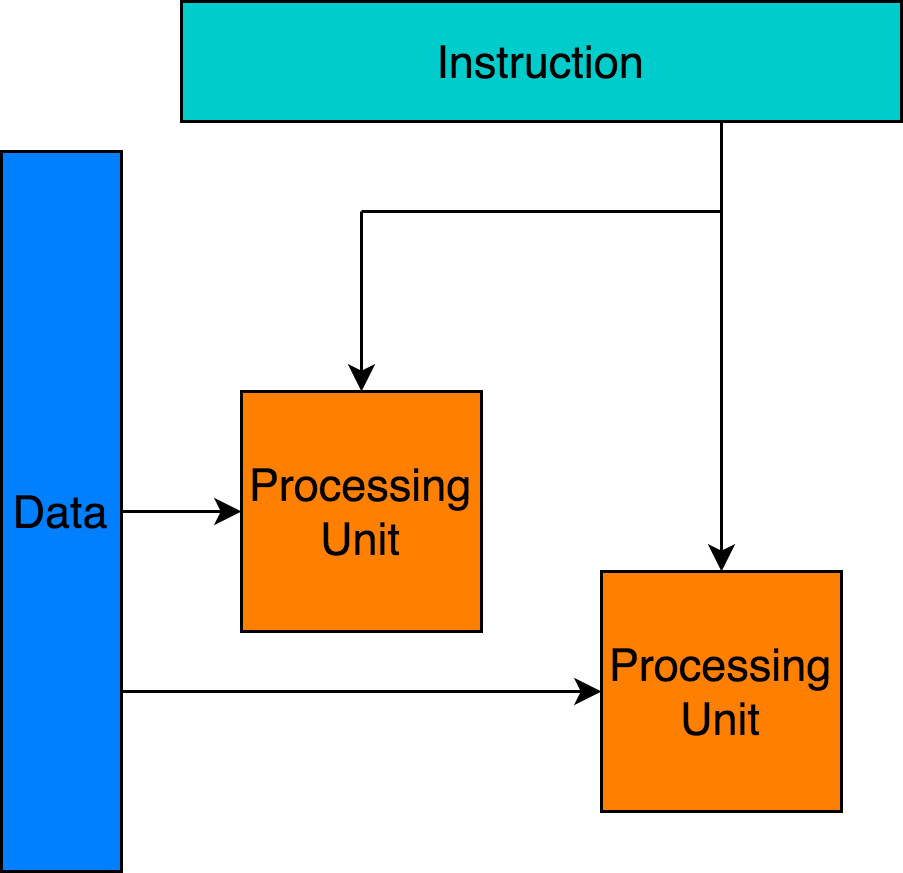
\includegraphics[width=5cm]{SIMD.png}
	\centering
	\caption{Single Instruction Multiple Data architecture}
	\end{figure}
	\item Multiple Instruction Stream, Single Data Stream (MISD): As the opposite of SIMD, this parallel organization is about multiple processors each have its own instruction stream while being fed with a common data stream. However, this kind of architecture is very uncommon compares to the other three~\cite{intro_parallel}.
	\begin{figure}[H]
	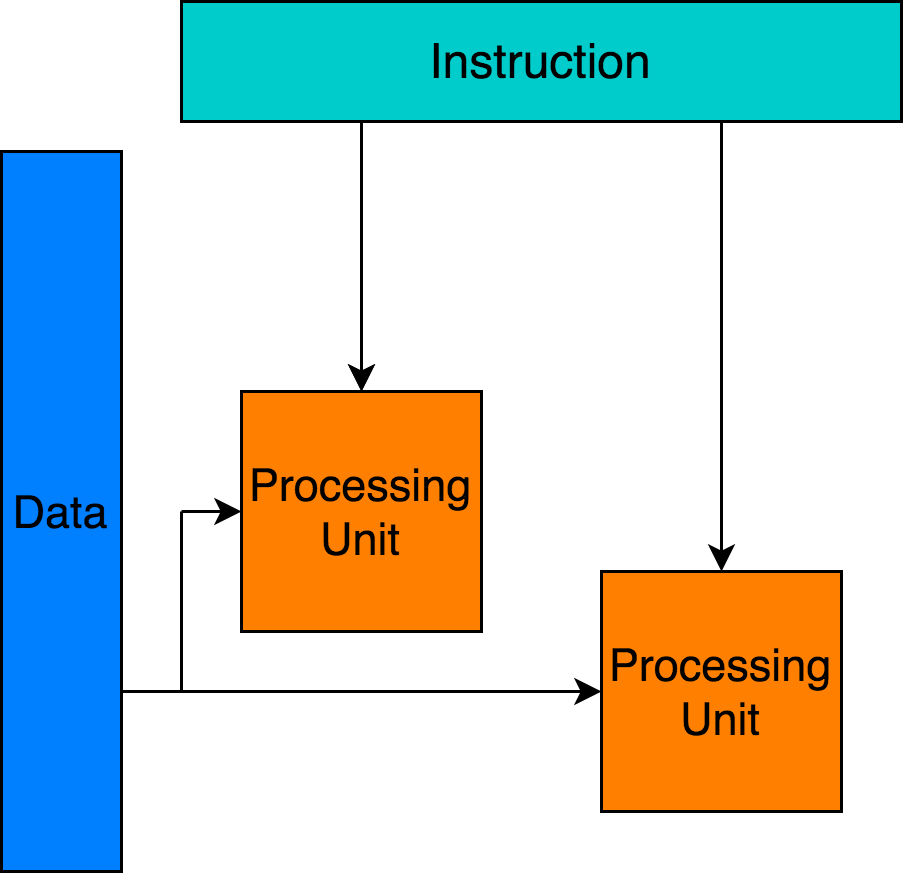
\includegraphics[width=5cm]{MISD.png}
	\centering
	\caption{Multiple Instruction Single Data architecture}
	\end{figure}
	\item Multiple Instruction Stream, Multiple Data Stream (MIMD): By far the most common class of parallel computer, especially in modern supercomputers, MIMD allows every processing units can have a different instruction stream and a different data stream. Different tasks can be handled by differnet processors, working on their own set of instructions and data. Because of this, task execution can be either synchronus or asynchronus, depending on the nature of the tasks~\cite{intro_parallel}.
	\begin{figure}[H]
	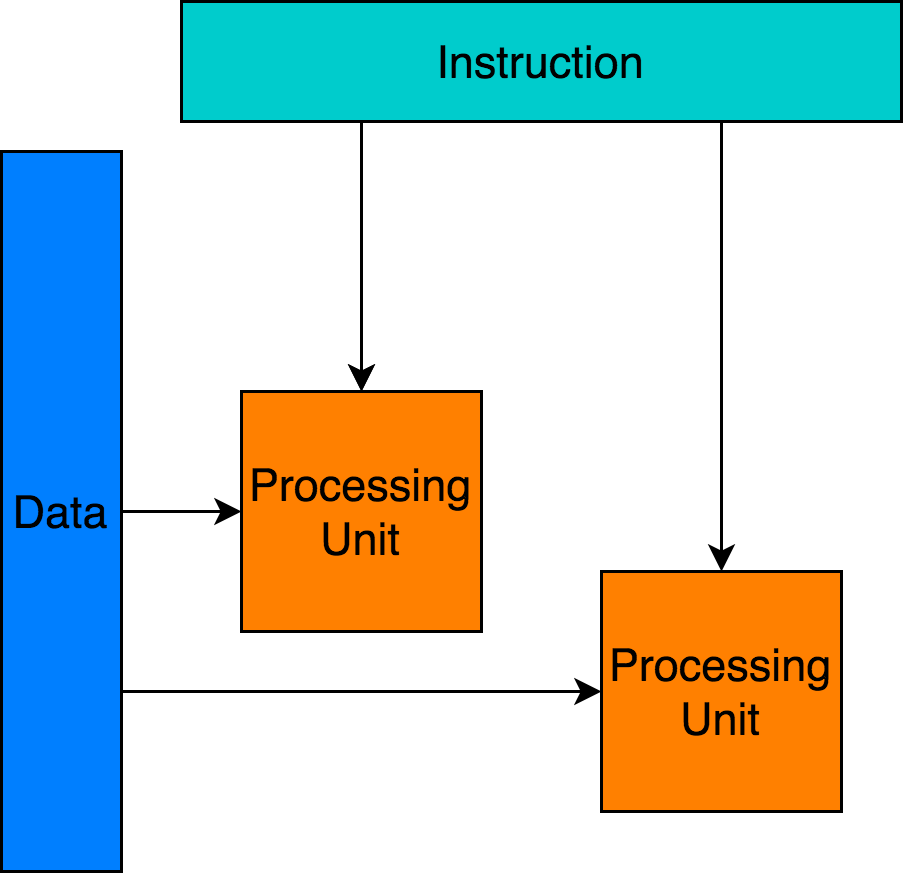
\includegraphics[width=5cm]{MIMD.png}
	\centering
	\caption{Multiple Instruction Multiple Data architecture}
	\end{figure}
\end{itemize}


\subsection{Maximum performance boost by Parallelization} 
While parallelism can provide better computation time compares to serial computing, there is a limit to how much parallelization can boost performance. Published in 1967, Gene M. Amdahl's paper, "Validity of single processing approach to achieving large scale computing capabilities", stated that there is a boundary in which how parallelism can speed up execution time, given there are always sequential overhead that slows down the computation tine and can't be spedup by applying parallelism~\cite{amdahl}. To represent this remark about the speedup, Admdahl gave a the following fomular: \\
\begin{equation}
Speedup = \frac{1}{r_s + \frac{r_p}{N}} ~\cite{amdahl} \\
\end{equation}
where r$_s$ stands for the serial portion of the code, the overhead that can't be paralleled. $r_p$ describes the parallel part of the program and $r_s + r_p = 1$. N illustrates the number of parallel processors. \\
~\\
In general, this equation implies that the speedup of parallel computing of N processors, compares to serial computing, can never be N times, because of the nature of the overhead as mentioned earlier. More importantly, if N ever reaches infinity, the speedup will equal to $\frac{1}{r_s}$. This number represents the bottle-neck of parallelism and is independent from the number of processors, meaning that the speedup also depends a lot on the program itself, how much of the code can and can't be paralellize. \\

\subsection{Drawbacks of Parallel Computing}
Despite all of its advantages by exploiting the potential of computer resource, both multicore processors and computers network, Parallel Computation, like all things, is not perfect and has can be a double-edge sword. As stated in the previous sections, speedup gained from parallelism does not align with the total number of processors or parallel workflows used in running the program. Because bottleneck factor comes from the program, it may be redundant to implement parallelism in some cases, where the performance gain might be insignificant, or even loses to serial computing. This is known as parallel slowdown. \\
~\\
Aside from the program's overhead produced by the serial portion of the code, other factors can affect slow down the computation time. Task scheduling plays a major role in this. In reality, for parallelism to function properly, the work needs to be divided and distributed to processors by the task scheduler, which will take time. The more the program has to be splitted, the more time it takes to for task scheduling to complete. Not to mention, more parallel tasks means that it will take more time to communicate between them. If the performance gain from parallel cannot justify these factors, a parallel slowdown is bounded to occur, thus rendering the parallelization useless. \\
~\\
How to implement parallelization is another drawback of this kind of computation. Generally, putting parallelism into practice is rather more complicated than people give it credit for. Not only does the programmer has to deal with the flow of instructions, he also has to take into account the data flow and avoid data dependencies, which agurably is the most problematic part of parallelism, where it is possible~\cite{intro_parallel}. Basically, data dependencies are when data needed from one instruction is related and depends on data of other instructions, thus making that part completely sequential and unparallelable. After successfully implemented parallelism, another challenge is to optimize the parallelization to yield the best possible performance compare to serial computing. \\
~\\
Another disadvantage of parallel computing that should be mentioned is the cost of computer resource. To effectively run paralleled softwares/programs, it usually requires a (or in some cases serveral) multicore CPU, which can be rather expensive, ranging from \$300 to \$1000 for a normal consumers multicore CPU. Higher grade CPU and system for High Perfomance Computing can cost thousands of dollar. Not only CPU can be costly but also dedicate GPUs and Memory as well. However, cost of HPC system is still feasible for many research institutes and individuals compares to supercomputer. \\


\section{Large Scale Parallelism: High Performance Computing system}
High Performance Computing system, or HPC for short, is designed to handle large computation problems, commonly seen in scientific researches, which require strong parallelism performance~\cite{hpc_status}. An HPC system can comprise of many computers, can be either in the same configuration or different specification from each other. In these machines, there are typically one or multiple Central Processing Units (CPUs), each has multiple cores. In addition, Memory that is much better in term of quality compares to consumer-grade product is installed in these kind of systems to ensure they have the best possible data access time. Moreover, for better parallel capability, computers in HPC system can be equipped with Graphic Processing Units (GPUs), specifically GPUs that support CUDA, a parallel computing platform and application programming interface designed by Nvidia. \\
~\\
Being one of the most powerful and flexible research tools to date, HPC systems are utilized to assist scientists in the study of real world events as mentioned in previous section~\cite{hpc_status}. While Personal Computers are very powerful on their own and can handle some advanced scientific programs, given that their components are top of their class, they still lack the horse-power needed to solve much heavier mathematical problems. HPC systems, on the other hand, provide the power of many computers combine, usually have better performance than those of Personal Computers, especially in parallel computation, thus accel in that regard. Because of this, HPCs are mostly seen in research institutes, data centers, or just about anywhere that is in need of and benefits from their parallel computational power. \\

\subsection{Cluster Computing System}

Cluster computing system is best described as a combination of stand-alone computers/workstations connected to each other locally via local network or internetwork to act as a single computer. Each machine in the Cluster system is considered as a node, having its own CPUs, whether it is single-core or multi-core, Memory, Network Interface hardware and other components. A cluster usually has 2 or more nodes integrated and can have shared storage for easy data accessing. To exchange data between with each other, nodes are connected to High Performance Network/Switch, for example Gigabit Ethernet or Infinity Band, and the Network Interface hardwares are in charge of sending and receiving node's data. Cluster computing is also referred to as High Performance Distributed computing~\cite{intro_cluster}. \\
% Illustration here
\begin{figure}[H]
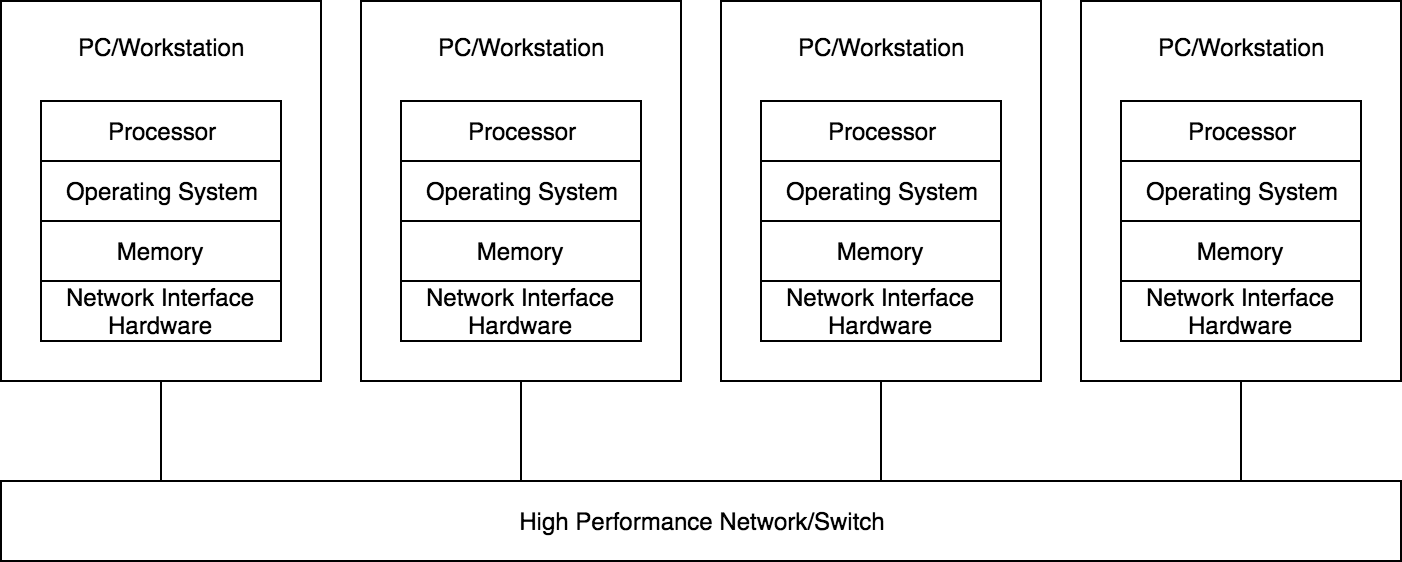
\includegraphics[width=12cm]{cluster.png}
\centering
\caption{Example of Cluster Computing Systems}
\end{figure}
~\\
Introduced by IBM in the 1960s as a concept, Cluster computer has exploded into the scene later down the line in the 1980s with the rise of current-time trends: high-performance microprocessors, high-speed network, standard tools for high performance distributed computing, and the increase in performance over price ratio in commodity computers components~\cite{ic_cluster}. As the technology has gotten more advanced as time goes, high-performance computer parts are readily available with fairly affordable price for their power, thus making Cluster computing systems that are built using off-the-shelf components an alternative to supercomputer, becoming an orthodox for high-performance, wide-throughput, readily-available parallel and distributed computing platform~\cite{intro_cluster}. \\

\subsection{Grid Computing System}

Grid computing gives an impression of simple and manageable yet very powerful virtual computer while in fact, Grid is a network of computers coupled together~\cite{redbook}. Unlike Cluster computers, which are locally connected independent computers, Grid Computing systems is a distributed computing infrastructure on a larger scale, not limited to local network or internetwork. Typically, Grid Computation's scale can be of that of geographical, in which each computer system that is part of the grid is placed in a different part of a city, country or even the world~\cite{grid_tech}. \\
~\\
Beside the fore-mentioned motivation of the need for parallel performance, Grid Computing also fulfills the purpose of removing the geographic barriers for collaboration on large-scale researches globally with minimum delay. Grid Computing provides means of managing distributed data access, processing data and storage, thus allowing data to be used by wider audiences. Sharing data is not the only thing Grid is capable of but also sharing computation resource, allow users to conduct experiments that are otherwise inefficient and impossible without it~\cite{intro_grid}. \\


\section{Local Scale Parallelism}

While Large Scale Parallelism system relies on splitting the work and have it done on many computers or processors, may it be single-core or multi-core, Local Scale Parallelism, on the other hand, depends entirely on the nature of the modern multi-core CPU. A multi-core CPU, as the name suggests, consists of 2 or more individual physical processing units, or cores, in a single package ~\cite{multicore}. These cores are coupled with each other by connecting to an internal bus of a shared cache memory within the CPU. Essentially, multicore CPU's architecture is designed following the MIMD architecture. Execution of multiple instructions at once is possible by feeding them into different cores, and each core, as a distinct processing unit, can handle its own set of data different from that of other cores~\cite{multicore}. \\
\begin{figure}[H]
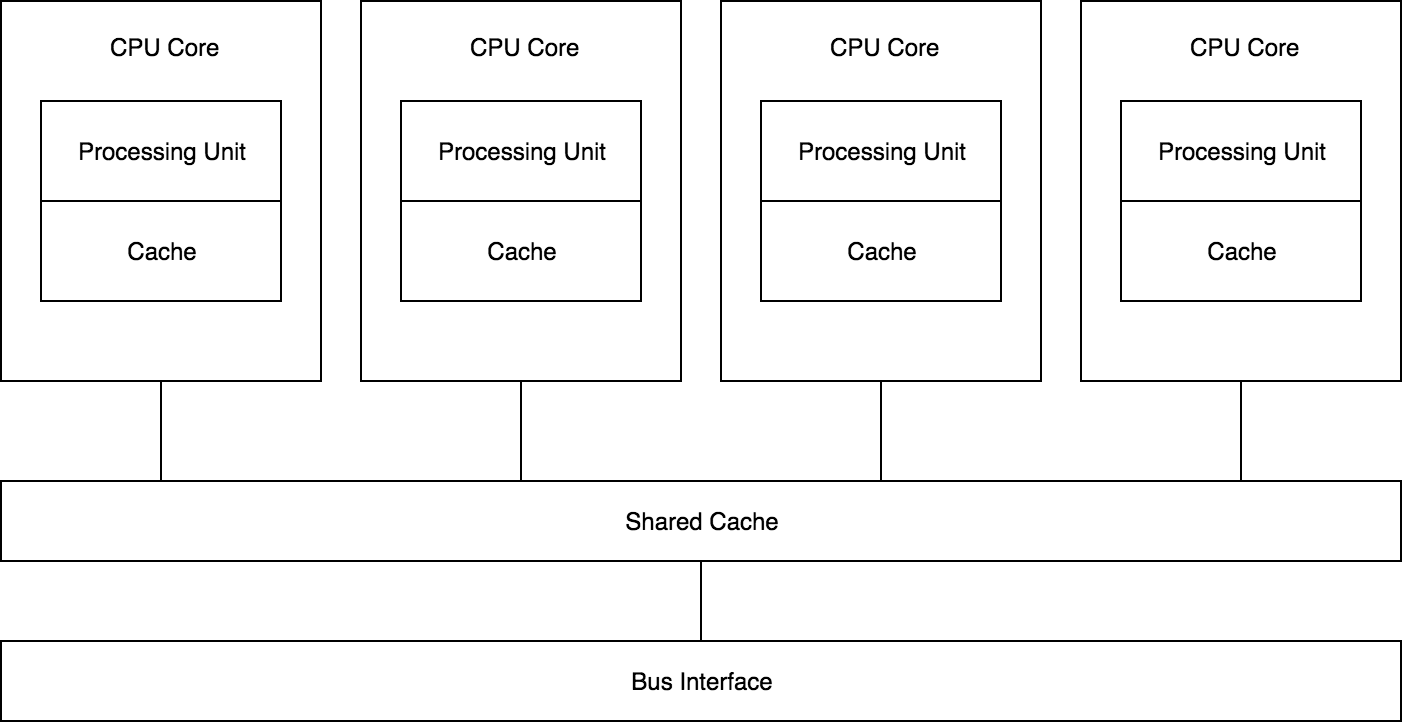
\includegraphics[width=11cm]{multi-core.png}
\centering
\caption{Example of a 4-core Processor}
\end{figure}
~\\
Current generation multi-core CPU also supports what is known as thread-level parallelism. This is kind of Local Scale Parallelism that executes tasks on individual threads of the CPU. A thread is basically a distinct process with its own instruction and data, and it can represent a part of a parallel program containing multiple processes. Thread-level parallelism is represented in the form of multithreading, having multiple threads sharing the same functional units of a processor~\cite{multicore}. For this reason, thread-level parallelism will increase computation performance, especially in demanding tasks that require doing multiple tasks at the same time, such as video rendering, which requires both raw computational power and multiple parallel throughputs. \\
%image of thread level parallel ?


% ----------------------- CHAPITRE ---------------------------

\chapter{Methodology}

Analyzing the source code of the program will give a good view of what is inside the program, and potentially find out where it is suitable for GPU parallel computation so that it can be implemented in the future. To investigate spots in RegCM that are likely to be benifited from GPU parallelism, profiling the software to locate what part of it takes the most computation time is the initial and crucial step. Next, data dependencies need to be detected in order avoid paralleling those section and hurt the performance of the program, or potentially break it. Finally, CPU thread-level is used to run RegCM as a proof of concept to see if there are any improvement in performance. While the initial goal of the internship is to have a demo of RegCM running parallel on GPU, but because of the time constrain, the best can be done was to evaluate the possibility of GPU parallelization. \\

\section{RegCM Installation}

As stated in the previous chapter, the main purpose of the intership is to investigate possible utilization of GPU parallelism within the Regional Climate Model. In order to achieve this goal, the source code of RegCM is required for analyzing the software and modify it for the demand of the intership. Furthermore, because the cluster used in REMOSAT lab is usually busy with running simulations, it would be best if RegCM can be installed in the ICTLab for easy accessibility. \\
~\\
Thankfully, RegCM is a open-source software, a term stands for softwares that are publicly accessible and anyone can share and/or revamp it. It is publicly available at: \url{http://gforge.ictp.it/gf/project/regcm/} . In this internship, version 4.3.5.6 is used because it is one of the most stable version and it is being ran by the REMOSAT laboratory. \\
~\\
The source code contains 3 main parts, 2 of those are for programs that pre-process the input data set and post-process the output of the simulation. The last part, and also the most important part, is the source code for RegCM, containing the main program of RegCM with its support modules. The simulation software is written in Fortran, a programming language that convenient for numeric and scientific computing. \\
~\\
Before the compilation of RegCM's source code, its prerequisite software needs to be installed. Those are Intel Fortran compiler, Hierarchical Data Format 5 (HDF5) and Network Common Data Form(NetCDF)-C 4 and NetCDF-Fortran 4. Moreover, for NetCDF, both C and Fortran version, to function properly, HDF5 is needed. In addition, supporting libraries, zlib and szip, are also mandatory. Finally, the Operating System used in this project is Debian, a Linux-distribution. \\
~\\
To start off RegCM installation process, Intel Fortran compiler needs to be installed first of all. This compiler is developed by Intel and is available in the Intel Parallel Studio XE development tools, designed specifically for High Performance Computing. This package is a commercial software, but Intel also offers free licenses for students and researchers. Simply follow the installation guide, enter a given product key, choose where to install and wait for the installer to complete. \\
~\\
After the installer is done, to complete the installation progress, enter the directory \\ \verb|intel_dir/bin/| and run 3 scripts, iccvars.sh, ifortvars.sh and compilervars.sh with parameter being the current system architecture, \verb|ia32| for 32-bit systems and \verb|intel64| for 64-bit systems. For example: 
\begin{center}
\begin{BVerbatim}
source compilervars.sh intel64
\end{BVerbatim}
\end{center}
Doing this will export the location contains the compiler executable files to the \verb|PATH| variable, thus enable the user to run these compilers without having to type the path of the compiler everytime. Lastly, export these variables: \\
\begin{center}
\begin{BVerbatim}
export CC=icc
export FC=ifort
\end{BVerbatim}
\end{center}
so that the default compiler for the system will those of Intel's. \\
~\\
Next, zlib and szip should be compiled and built, respectively. Both of these libraries are required for installing HDF5 and NetCDF later on. They are available at \url{https://zlib.net/} and \url{http://www.compressconsult.com/szip/}. In order to install these libraries, simply run the following commands
\begin{center}
\begin{BVerbatim}
./configure --prefix=/directory/to/install
make
make install
\end{BVerbatim}
\end{center}
each time for each library. The \verb|--prefix=/directory/to/install| is for installing libraries in a different folder other than the default \verb|/usr/local/| folder. \\
~\\
HDF5's source code can be obtained at \url{https://support.hdfgroup.org/HDF5/release/obtain5.html}. The version was used in the ICTLab's cluster was HDF5-1.8.16. After the source code was extracted from the archive, the installation progress takes 3 commands, just like with zlib or szip:
\begin{center}
\begin{BVerbatim}
./configure --prefix=/directory/to/install --with-zlib=/zlib-dir
	--with-szip=/installed/szip/dir --enable-parallel
make
make install
\end{BVerbatim}
\end{center}
Nonetheless, it is crucial to state in the configure command where were szip and zlib installed, if they were not installed in the default folder. The \verb|--enable-parallel| paramemter will tell the configuration process to look for MPI-IO and MPI support files, which was installed previously along with Intel Parallel Studio. \\
~\\
To install the last prerequisite, and undoubtedly the most important one, NetCDF, there are a couple of things to note. First, there are two versions of NetCDF, one using C interface and the other uses Fortran, and both are required. Second, unlike HDF5's install process where the user can state the location of the libraries by configuration's parameter, NetCDF requires the user to specify libraries's path to \verb|CPPFLAGS|, \verb|LDFLAGS| and \verb|LD_LIBRARY_PATH|. Source code for NetCDF is available at \url{https://www.unidata.ucar.edu/downloads/netcdf/index.jsp}. Again, the version of NetCDF-C and NetCDF-Fortran was used in this project are those that are used by REMOSAT, NetCDF-C 4.4.0 and NetCDF-Fortran 4.4.3. NetCDF is installed in the following order: NetCDF-C, then NetCDF-Fortran. \\
~\\
To compile and build NetCDF-C, the initial step, as stated previously, libraries's path needs to be added to environement variables
\begin{center}
\begin{BVerbatim}
export CXX=icpc
export CPPFLAGS="-I/zlib-dir/inlcude -I/hdf-dir/include"
export LDFLAGS="-L/zlib-dir/lib -L/hdf-dir/lib"
export LD_LIBRARY_PATH=/zlib-dir/lib:/hdf-dir/lib:$LD_LIBRARY_PATH
\end{BVerbatim}
\end{center}
After setting environment variables is complete, proceed to configure and install NetCDF-C
\begin{center}
\begin{BVerbatim}
./configure --prefix=/directory/to/install
make
make install
\end{BVerbatim}
\end{center}
With NetCDF-Fortran, the environment variables needs to be updated with NetCDF-C's path
\begin{center}
\begin{BVerbatim}
export CPPFLAGS="-I/zlib-dir/inlcude -I/hdf-dir/include 
	-I/netcdf-c-dir/include"
export LDFLAGS="-L/zlib-dir/lib -L/hdf-dir/lib 
	-L/netcdf-c-dir/lib -lnetcdf"
export LD_LIBRARY_PATH=/netcdf-c-dir/lib:$LD_LIBRARY_PATH
\end{BVerbatim}
\end{center}
Following that, start the install process, which is simillar to NetCDF-C's, and once finished, all needed compoments are installed and RegCM are ready to be configured and built. \\
~\\
In order to install RegCM, these compiler variables have to be exported:
\begin{center}
\begin{BVerbatim}
export I_MPI_CC=icc
export I_MPI_CXX=icpc
export I_MPI_FC=ifort
export I_MPI_F77=ifort
export I_MPI_F90=ifort
\end{BVerbatim}
\end{center}
Previously mentioned, RegCM has full support for Message Passing Interface, or MPI, so MPI compilers are necessary. Because the standard compiler used to build RegCM are those of Intel's, the MPI compiler are required to match those as well, or the installation process won't be successful. The installation procedure follows the above normally, though no prefix for installation folder is needed, since all the compiled binary files of RegCM are stored within the newly created \verb|bin| folder inside the source code folder. \\
~\\
The final step of the RegCM Installation Process is to create a working environment for RegCM. This starts with making a new folder to hold the binary files, input and output of simulations. Next, 2 more folders need to be inside the newly created folder, one to contain the pre-processed data for the input of RegCM, the other is the output directory of the simulation. Lastly, a symlink is formed to link the current folder to the bin folder of RegCM. For example:
\begin{center}
\begin{BVerbatim}
ln -sf /RegCM-source-code-folder/bin
\end{BVerbatim}
\end{center}
This link will allow the current folder to contain a reference to the \verb|bin| folder that was created earlier during the installation process. \\
~\\
During initial installation of the software in the internship, some difficulties was encountered. There was a lack of in-depth information on how to install the software and its prerequisites. The User Manual provided by the software's author did not specify what compiler should be utilized, what version of the dependencies is needed. At first, the programs was installed with standard Linux gcc and gfortran compilers but many errors occurred along the way. Through many trial-and-errors and with the help of the REMOSAT laboratory, RegCM was finally installed into the cluster system of USTH ICTLab, though it was very time-consuming and took the most amount of time in the internship. Nonetheless, it was worth putting effort into to ensure a proper working environment. \\

\section{Profiling RegCM}
The first step, and arguably the most crucial step of all, is to profile the Regional Climate Model, to see which part of the program takes the most out of execution, and from there on, as a starting line, dig in further into the program, repeat the process to find spots that are suitable for implementing parallelization. Characteristic that should be on the look out are for-loops with high number of iterations and simple mathematic computation. \\
~\\
To profile the simulation, a subroutine is written to record the current in millisecond and put it at just before the start and right after the end of a designated section of code that need to be profiled to note down the start time and finish time of that section. The time duration it takes to execute that section is the subtraction of the two above values. \\
~\\
Fortran provides a subroutine to retrieve information on computer's date and time in the form of an array, containing data on current year, month, date, time zone, hour, minute, second and millisecond. The subroutine is written as follow:
\begin{center}
\begin{BVerbatim}
subroutine time_in_ms(rTime)
    integer(ik8) :: values(8)
    real(rk16) :: rTime
    call date_and_time(values=values)
    !Hours to minutes  
    rTime = ( values(5) ) * 60
    !Minutes to Second
    rTime = ( rTime + values(6) ) *60
    !Second to ms 
    rTime = ( rTime + values(7) ) *1e3
    !adding ms 
    rTime = rTime + values(8)
 end subroutine time_in_ms
\end{BVerbatim}
\end{center}
In order to get the current time in millisecond, a conversion from other time units to millisecond is needed. Under the premise that no subroutine in RegCM should take more than 24 hours for one run, there are only 3 time units that require to be converted, hour, minute, and second and add all of them up to get the final result.  \\
~\\
In the source code, the file named \verb|mod_regcm_interface.F90| contains the main program of RegCM, initializing the simulation, calling other subroutines from other modules for calculations. These computation of RegCM simulation can be seen in \verb|RegCM_run| subroutine, thus a good place to start. In this subroutine, there is a while-loop, running steps of simulation's duration, containing calls for computing model's tendencies, structure's manipulation, solar declination angle, new boundary conditions reading and filling boundary with input values and tendencies. Measuring the execution time of these subroutines that was called by the main program will give a general look at what takes the most time. The table below shows how the profiling turned out for different simulation's duration: \\
\begin{table}[H]
\centering
\resizebox{\textwidth}{!}{%
\begin{tabular}{@{}lrrrrrrrr@{}}
\toprule
\multirow{2}{*}{} & \multicolumn{2}{c}{2 months}         & \multicolumn{2}{c}{4 months}         & \multicolumn{2}{c}{6 months}         & \multicolumn{2}{c}{8 months}         \\ \cmidrule(l){2-9} 
                  & Total Exe. Time(ms) & Percentage(\%) & Total Exe. Time(ms) & Percentage(\%) & Total Exe. Time(ms) & Percentage(\%) & Total Exe. Time(ms) & Percentage(\%) \\ \cmidrule(r){1-1}
Tendencies        & 1723176             & 94.38          & 3557137             & 94.39          & 5379873             & 94.39          & 7222206             & 94.38          \\
Split Mode        & 92382               & 5.06           & 188920              & 5.01           & 286476              & 5.03           & 384908              & 5.03           \\
Solar             & 1                   & 5.48E-05       & 5                   & 1.33E-04       & 6                   & 1.05E-04       & 8                   & 1.05E-04       \\
New Boundary      & 523                 & 0.03           & 1159                & 0.03           & 1718                & 0.03           & 2352                & 0.03           \\
Fill Boundary     & 1751                & 0.10           & 16021               & 0.43           & 23906               & 0.42           & 32484               & 0.42           \\
Misc.             & 8041                & 0.44           & 5167                & 0.14           & 7832                & 0.14           & 10397               & 0.14           \\
RegCM             & \multicolumn{2}{r}{1825874}          & \multicolumn{2}{r}{3768409}          & \multicolumn{2}{r}{5699811}          & \multicolumn{2}{r}{7652355}          \\ \bottomrule
\end{tabular}%
}
\caption{Result of profiling different subroutines in different simulation duration}
\end{table} 
~\\
It can be seen easily that calculating tendencies for the model takes a tremendous amount of time, occupied aroung 90\% of the whole simulation time. This is a clear sign that the subroutine responsibles for these calculations should be investigated further. \\
~\\
Inside \verb|tend| subroutine of \verb|mod_tendency.F90| file, which handle the model's tendencies calculation, there are 70 main for-loops, all of which are nested with other different for-loops. These main for-loops will be the focus of profiling further \verb|tend| subroutine, as they fit the above wanted characteristics. Again, the profiling process is done much like the same with the first one. \\
~\\
However, things are a little differnet in this case because of 2 key reasons. First, the \verb|tend| subroutine is looped thousand of time, based on the model's simulation time, thus generates lots of data when logging to see the execution time of the loops. Second, there are some loops in this subroutine that are not executed in the process, one may execute in an iteration of the program while not being touched in other iterations. Because of this, it is hard to keep track of all these for-loops, in which knowing when they will occur in the massive amounts simulation's iterations. In order to overcome this problem, 10 profiling results belong to 10 iterations of RegCM will be choosen randomly, and the average execution time of each for-loops inside \verb|tend| will be calculated based on the chosen 10 to see which take the most time. Below are the result: \\
\begin{table}[H]
\centering
%\resizebox{\textwidth}{!}{%
\begin{tabular}{@{}rr@{}}
\toprule
Loop No. & Average Execution Time(ms) \\ \midrule
48       & 2.7                        \\
60       & 1.4                        \\
52       & 1.3                        \\
19       & 0.7                        \\
26       & 0.7                        \\ \bottomrule
\end{tabular}%
%}
\caption{Top 5 most time consuming for-loops in tend subroutine on average}
\end{table}
~\\
The result shows interesting information. While these 5 for-loops are those that take the most time to execute, their average time is very small, capping at only 2.7 ms. Add in the fact that tendencies has the most performance time, these numbers mean that these loops, while big in number of iterations, take very little time to complete. \\
~\\
These 5 for-loops that was shown in the result will be choosen to investigate possible data dependencies, then to try parallelize them to see if there are any improvement in performance. However, one thing to note is that since the number of iterations is enormous, 10 results from randomly choosen iteration might be not enough to clearly asset this problem. Further and deeper inspection of profiling is needed in the future. \\

\section{Investigate possible Data Dependencies}

Data Dependencies, or Data Hazards means that an instruction requires data that is the result of a previous instructrion. Detecting Data Dependencies is a crucial task in implementing parallelization, since data dependencies can harm the parallel computing's performance. The outcome if Data Dependencies is not handled properly is that the parallel program will perform worse since there are parts of the program that has to wait for data to be produced by previous section, thus making parallelization useless while processor still has to schedule the work. \\
~\\
After examined the source code of the 5 fore-mentioned for-loops, it appeared to the naked eye that none of them has any data dependencies. All the loops seem to not using any input that relies on the result produced in previous iterations. However, to be fully confident that there exists no data hazards, inspecting the source code is insufficient, especially with code from other authors since the one doing code's analysis often is foreign to the source code and cannot be sure of the intention of the author. Investigation of this subject will be clearer once these for-loops are parallelize using OpenMP, which will be cover in the next section. This action will allow the observation of each loop's behavior to draw a better conclusion. \\

\section{Open Multi-Processing - OpenMP}

Open Multi-Processing, or OpenMP for short, is an API(Application Programming Interface) for C/C++ and Fortran, contains compiler directives, libraries routine and environment variables that enable high-level parallelism~\cite{ompfaq}. The selling point of OpenMP is that while most of the time, without it, programmers struggle to distribute workload in processors, and to solve the problem of non-standardization of processors's clock speed, the API simplify these programming processes, giving specific instructions automatically to the processors, thus reduced the work need to be done when parallelizing a program. Because of its ease of parallel implementation, existing serialize code can be parallelize with little effort to test parallel compatability of sections of code~\cite{omp_intro}. \\
~\\
%add OMP directive, and use compiler flag and link library
To use OpenMP Parallelization API, simply add the OpenMP directives to sections that need to be parallelize. In this project, the 2 directives that were used are: 
\begin{center}
\begin{BVerbatim}
!$OMP PARALLEL DO
!$OMP END PARALLEL DO
\end{BVerbatim}
\end{center}
These 2 directives were put, respectively, at the beginning and the end of each for-loop, telling the compiler that these sections are to be run in parallel. Lastly, to compile code that use OpenMP, one needs to add the compiler flag and link the library of OpenMP when compiling the code. Depends on the compiler, the flag can vary. Here, the OpenMP flag for Intel compiler is \verb|-fopenmp|. Linking OpenMP library are more uniform by adding \verb|-liopm5| before compilation. \\
~\\
%talk about those loops that failed
It is interesting to note that adding OpenMP directives to loop number 19 and number 26 in \verb|tend| subroutine, RegCM will crash and generate fatal error. It is suspected that these 2 loops has data dependencies of their own that causes the crash to happen. For further testing of potential parallelization of RegCM, the 2 mentioned loops were removed from the scope of the test to ensure RegCM functions normally. 

% ----------------------- CHAPITRE ---------------------------

\chapter{Results}


This part must contain the result of the method/algoritm/system developed during the internship. \\

This part must also include comparisons with the state of the art.\\

Use tables, figures, graphics to illustrate your results. \\ 

Comment your results, and explain the context used to obtain these results.







% ----------------------- CHAPITRE ---------------------------

\chapter{Conclusion}


You can recall the problematic of your internship and explain if you have solved all the problem or not. \\

Recall the methods used and your contribution.\\

Recall the results obtained and explain the quality of your results in comparison with the state of the art.\\


Give some perspectives of your work.



% ----------------------- BIBLIOGRAPHIE ---------------------------

\bibliography{Biblio}
\bibliographystyle{unsrt}

% ----------------------- ANNEXES ---------------------------

\appendix

\appendix

\chapter{Detail about ...}

In this part, you can add more details about some technical parts which need too much detailed impossible to include in the report body of your report








\chapter{Mathematical demonstration}

If necessary, you can add appendix to show mathematical demonstrations.





\end{document}
